\documentclass[11pt]{article}
\usepackage{fullpage}
\usepackage{amsthm}
\usepackage{amsmath} \usepackage{amssymb}
\usepackage{graphicx}

\graphicspath{ {./imgs/} }

\setlength{\parindent}{0pt}

\title{Performance Engineering (CO339)}
\author{Michael Tsang}

\newtheorem{defn}{Definition}
\newtheorem{eg}{Example}
\newtheorem{theo}{Theorem}
\newtheorem{lem}{Lemma}

\begin{document}

\maketitle

\section{Motivation}
\textit{Performance engineering encompasses the techniques applied during a systems development life cycle to ensure the \textbf{non-functional requirements for performance} will be met.}

\subsection{System}
\begin{defn}
  A regularly interacting or independent group of items forming a unified whole.
\end{defn}

\begin{itemize}
  \item Made up from \textbf{components} that interact to achieve a \textbf{greater goal}.
  \item Applicable to many situations (generic).
  \item Goal is domain-agnostic.
  \item Components serve a data-management purpose, not a domain purpose.
\end{itemize}

\subsection{Success}
To define success, we need to define a \textbf{metric} and a \textbf{threshold}.

The metric could be throughput, latency, scalability, memory usage, energy consumption, TCO, elasticity, efficiency\dots.

We have two options when declaring success:
\begin{itemize}
  \item Setting an optimization \textbf{budget}.
  \item Setting an optimization \textbf{target}.
\end{itemize}

\subsection{Defining the Target}

\subsubsection{\textit{SMART} Requirements}
\begin{itemize}
  \item \textbf{Specific} - state exactly what is acceptable in numeric terms.
  \item \textbf{Measureable} - make sure what is stated can be measured.
  \item \textbf{Acceptable} - rigorous enough to guarantee success in reality.
  \item \textbf{Realizable} - lenient enough to allow implementation.
  \item \textbf{Thorough} - all necessary aspects of the system are specified.
\end{itemize}

\subsubsection{Quality-of-Service (QoS) Objectives}
\begin{defn}
  Statistical properties of a metric that shall hold for the system.
\end{defn}
\begin{itemize}
  \item Can include pre-conditions.
  \item Could conflict with functional requirements.
\end{itemize}

\begin{eg}
  The framerate of the game will, on average, be higher than 60 frames/s if run on a GPU with 50 GFlops or more.
\end{eg}

\subsubsection{Service-Level Agreements (SLA)}
\begin{defn}
  Formal, legal contracts specifying QoS objectives, as well as penalities for violations.
\end{defn}
\begin{itemize}
  \item Needs enforcement through monitoring.
\end{itemize}

\begin{eg}
  Trading orders shall not exceed 1ms response time. 
  In case of violation, the user is eligible for a 10\% credit towards fees.
\end{eg}


\subsubsection{Monitoring}
\begin{itemize}
  \item Constant monitoring is required to enforce SLAs.
    \begin{itemize}
      \item Observe system performance.
      \item Collect statistics.
      \item Analyze data.
      \item Report SLA violations.
    \end{itemize}
  \item Monitoring can incur costs $\rightarrow$ often not continuous.
\end{itemize}

\subsection{Fulfilling Performance Requirements}
Examples of performance evaluation techniques are:
\begin{itemize}
  \item Simulation.
  \item Measuring.
  \item Analytical modeling.
  \item Hybrids, e.g.\ measure then model; model and simulate\dots
\end{itemize}

\subsubsection{Measuring}
\begin{itemize}
  \item Performed on a prototype or on the final system.
  \item Closely related to monitoring, promises good accuracy.
  \item Often based on instrumentation.
  \item Costly, and can be difficult.
\end{itemize}

\subsubsection{Benchmark}
Two step process:
\begin{enumerate}
  \item Get the system into a predefined state.
  \item Perform a series of operations (the workload) while measuring performance.
\end{enumerate}

\subsubsection{Workloads}
\begin{itemize}
  \item \textbf{Batch} workloads:
    \begin{itemize}
      \item Program has access to entire batch at start.
      \item Useful when metric is throughput.
      \item Simple, generator performance does not matter.
    \end{itemize}
  \item \textbf{Interactive} workloads:
    \begin{itemize}
      \item Work generated piece by piece (randomly).
      \item Useful when metric is latency.
      \item Generator should be at least as fast as system under evaluation.
    \end{itemize}
  \item \textbf{Hybrids}:
    \begin{itemize}
      \item Sample random queries from a predefined work set.
    \end{itemize}
\end{itemize}

\subsubsection{Parameters}
\begin{itemize}
  \item \textbf{System Parameters} - generally do not change (e.g.\ caches; CPU instruction costs).
  \item \textbf{Workload Parameters} - may change, even while system is running (e.g.\ users; available memory).
\end{itemize}

\subsection{Interpreting Performance Metrics}
\begin{itemize}
  \item A single number is generally meaningless, there is too much noise in modern computer systems.
  \item We aggregate multiple runs and report some measure of variance - \textbf{statistics}.
  \item We can represent statistics with charts, e.g.\ box and whisker charts.
\end{itemize}

\begin{defn}
  \textbf{Utilization} is the percentage of a resource that is used to perform a service.
\end{defn}

\begin{defn}
  \textbf A {bottleneck} is the resource with the highest utilization.
\end{defn}

\subsection{Improving Performance}
We compare alternative designs (\textbf{development}) or select a close-to-optimal value for a parameter (\textbf{tuning}).

\subsubsection{Analytical Modeling}
\begin{defn}
  A set of equations describing the mathematical relationship between performance parameters and performance metrics.
\end{defn}

We model a dynamic system using \textbf{static equations}.
This is the key distinction to simulation, which is dynamic.

Analytical models are fast and allow what-if analysis, which simplifies tuning.
If we can build an analytical model, we have understood the system.

\subsubsection{Parameter Tuning}
Workload parameters are not usually under our control.
\begin{defn}
  \textbf{Parameter tuning} involves finding the vector in the parameter space that either \textbf{minimizes the resource consumption} or \textbf{maximizes a performance metric}. 
\end{defn}
We need to explore the parameter space, which is expensive.
Analytical models help to accelerate this process immensely.

\subsubsection{Tradeoffs}
Sometimes consumption of an expensive or non-scalable resource can be reduced by using more of a cheaper one - this may require changes to the system.

\section{Performance Profiling and Tracing}
\begin{defn}
  A \textbf{profile} is a graphical or other representation of information relating to particular chracteristics of something, recorded in quantified form.
\end{defn}
We characterize the system in terms of the time it spends in certain states.

The system can be applied to any level: CPU, OS, distributed, application, etc.

We profile in order to:
\begin{itemize}
  \item Identify the critical path.
  \item Identify bottlenecks.
  \item Tune.
\end{itemize}

\subsection{Events}
An \textbf{event} is some change of the system state, this depends on what needs to be measured.
There are two types:
\begin{itemize}
  \item \textbf{Simple/atomic events} - a package sent, instruction executed, address loaded from memory, a clock tick, etc.
  \item \textbf{Complex events} - cache line evicted from L1 to L2 cache, instruction aborted due to miss-speculation.
\end{itemize}

\subsubsection{Collecting Events}
\begin{itemize}
  \item \textbf{Event-based/event-counting}:
    \begin{itemize}
      \item Count events on occurence.
      \item Little overhead, limited information.
    \end{itemize}
  \item \textbf{Tracing}:
    \begin{itemize}
      \item Keep state for every event.
      \item Higher overhead, more information.
    \end{itemize}
  \item \textbf{Sampling}:
    \begin{itemize}
      \item Keep state in \textbf{intervals}.
      \item Inaccurate and non-deterministic.
      \item Interval size $1$ makes sampling equal to event-based profiling.
    \end{itemize}
  \item (\textbf{Indirect}:)
    \begin{itemize}
      \item Counting events that dominate (correlate with) others (if this event occurs, then other events will occur - we consider the \textit{other events}).
      \item Can be used to reduce overhead.
      \item Accuracy depends on the event and indirection.
    \end{itemize}
\end{itemize}

\subsection{Profile}
An aggregrate over the events of a specific metric:
\begin{itemize}
  \item \textbf{Global aggregate} - total cache misses, total CPU cycles, etc.
  \item \textbf{Broken down} by some other event - cycles per instruction, cache misses by line of code.
\end{itemize}

\subsection{Trace}
A complete log of every state the system has ever been in (in a period of interest):
\begin{itemize}
  \item Characterized by the events.
  \item There is a total order of events.
  \item \textit{Stream of events}.
\end{itemize}
By aggregating, we can turn this into a profile.

\subsection{Classification}
\begin{itemize}
  \item Sampling rate (interval) $=1$:
    \begin{itemize}
      \item With payload - \textbf{tracing}.
      \item Without payload - \textbf{event-based profiling}.
    \end{itemize}
  \item Sampling rate (interval) $>1$:
  \begin{itemize}
    \item \textbf{Sampling}.
  \end{itemize}
\end{itemize}

\subsection{Collection Framework}
Our framework consists of two components:
\begin{itemize}
  \item \textbf{Generator} - produces events; usually online, part of the runtime environment.
  \item \textbf{Consumer} - producing visualisation or profile from trace; offline or online.
\end{itemize}

\subsection{Time}
\begin{itemize}
  \item Computer clocks are not very accurate.
  \item We use reference cycles as a proxy metric.
  \item Any event may be used to define intervals.
\end{itemize}

\subsection{Quantization Errors}
\begin{itemize}
  \item The interval resolution is limited.
  \item However, time is continuous.
  \item This introduces errors as costs may be attributed to the wrong instruction.
\end{itemize}

\subsection{Call Stack}
\subsubsection{Call Stack Tracing}
Recording the entire call stack is quite expensive:
\begin{itemize}
  \item Stack needs to be walked, pointers need chasing.
  \item Call stacks can be deep.
  \item Record must be written to memory.
\end{itemize}

\subsubsection{Call Stack Sampling}
\begin{itemize}
  \item Limited accuracy, but better performance.
  \item Less pertubation.
\end{itemize}

\subsubsection{Flame Graphs}
\begin{figure}[htb!]
  \centering
  \caption{A flame graph.}
  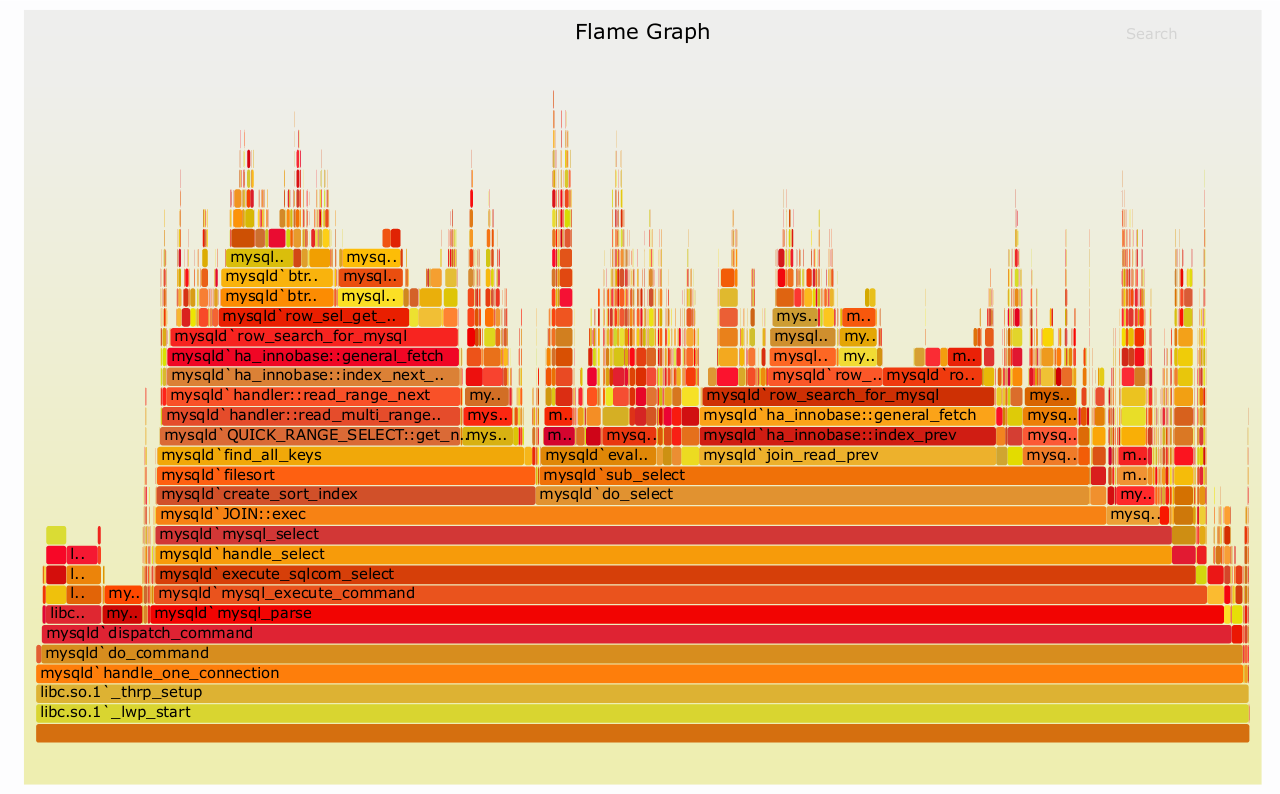
\includegraphics[width=\textwidth]{flamegraph}
\end{figure}
The $x$-axis shows the stack profile population, sorted alphabetically - it does not show the passage of time.
The $y$-axis shows the stack depth, counting from zero at the bottom.

Each rectangle is a stack frame; the wider the frame, the more often it was present in the stacks.
The top edge shows what is on-CPU, beneath is its ancestry.

\subsection{Event Sources}
We require event sources to be:
\begin{itemize}
  \item \textbf{Detailed} - as much information as we need.
  \item \textbf{Accurate} - reliable measurements.
  \item \textbf{Little perturbation} - does not change the performance of the system during analysis (often inversely proportional to accuracy).
\end{itemize}

We can get events from:
\begin{itemize}
  \item \textbf{Software} - e.g.\ OS kernel counts, library logging, compiler instrumentation.
  \item \textbf{Hardware} - e.g.\ performance counter.
  \item \textbf{Emulator} - hybrid of software and hardware; minimal perturbation but not scalable.
\end{itemize}

\subsection{Instrumentation}
We augment the program with event logging code.
\begin{itemize}
  \item Advantages:
    \begin{itemize}
      \item No need for hardware support.
      \item Flexible.
    \end{itemize}
  \item Disadvantages:
    \begin{itemize}
      \item High overhead.
      \item High perturbation.
    \end{itemize}
\end{itemize}
We need to decide on what events we should collect.

There are three approaches to instrumentation:
\begin{itemize}
  \item Manual instrumentation.
  \item Automatic source-level instrumentation.
  \item \textbf{Automatic binary instrumentation} - could be static (compile-time), dynamic (runtime), or as a hybrid.
\end{itemize}

\subsubsection{Manual Instrumentation}
\texttt{printf} logging.
\begin{itemize}
  \item Advantages:
    \begin{itemize}
      \item Fine control.
      \item No need for support from hardware or compiler.
    \end{itemize}
  \item Disadvantages:
    \begin{itemize}
      \item High overhead.
      \item Disabled for release build.
    \end{itemize}
\end{itemize}

\subsubsection{Automatic Instrumentation}
Usually supported by the compiler; source-to-source rewriting is possible.
\begin{itemize}
  \item Advantages:
    \begin{itemize}
      \item Delegating expertise of what needs to be logged to the compiler.
    \end{itemize}
  \item Disadvantages:
    \begin{itemize}
      \item Less control.
      \item Need for compiler support.
    \end{itemize}
\end{itemize}

\subsubsection{Binary Instrumentation}
\begin{itemize}
  \item \textbf{Static}:
    \begin{itemize}
      \item No magic; simple and portable.
      \item Instrumentation overhead can be accessed from binary.
    \end{itemize}
  \item \textbf{Dynamic}:
    \begin{itemize}
      \item No recompilation.
      \item Can be performed on a running process.
      \item Works with JiT-code.
    \end{itemize}
\end{itemize}

\subsection{Performance Counting}
\begin{itemize}
  \item \textbf{Software Performance Counters} (OS):
    \begin{itemize}
      \item e.g.\ network packages sent, virtual memory operations.
      \item Only of secondary interest.
    \end{itemize}
  \item \textbf{Hardware Performance Counters}:
    \begin{itemize}
      \item Fixed number can be active at runtime.
      \item Usually buggy, unmaintained, and poorly documented, with poor accuracy.
      \item Common counters usually okay.
    \end{itemize}
\end{itemize}

\section{Top-down Microarchitecture Analysis Method (TMAM)}
The TMAM identifies performance bottlenecks in out-of-order cores.
Bottlenecks are classified correlating to major functional blocks of modern out-of-order microarchitectures, with four main categories of pipeline-slots:
\begin{itemize}
  \item \textbf{Front End Bound}.
  \item \textbf{Back End Bound}.
  \item \textbf{Bad Speculation}.
  \item \textbf{Retiring}.
\end{itemize}
the latter two denoting non-stalled slots, while the former two stalled slots.

\begin{figure}[htb!]
  \centering
  \caption{Decision tree for categorizing slots.}
  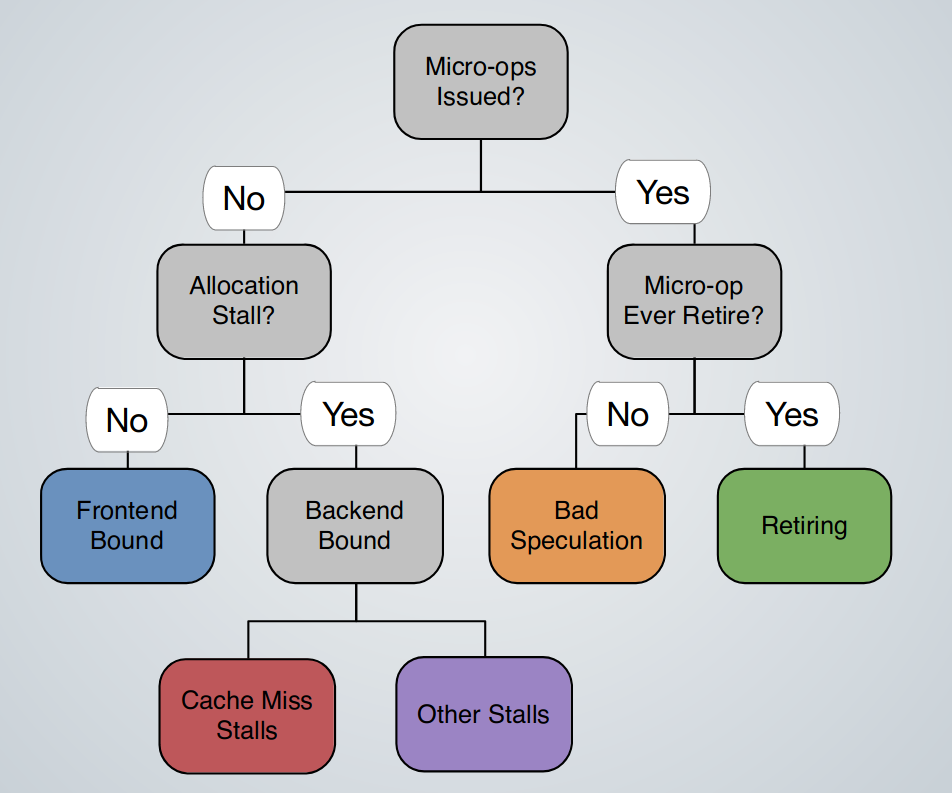
\includegraphics[scale=0.3]{tmam}
\end{figure}

If a slot is being utilized, it is classified as either Retiring or Bad Speculation, depending on if it eventually retires.
Otherwise they are classified as Back End Bound if the back-end is unable to accept more operations, or Front End Bound if there were no operations (uops) delivered while there was no back-end stall.

\subsection{Front End Bound}
\begin{defn}
  The \textbf{front end} is the portion of the pipeline where the branch predictor predicts the next address to fetch, fetches, parses, and decodes into micro-ops that can be executed later by the back end.
\end{defn}

\begin{defn}
  \textbf{Front End Bound} denotes when the fron end of the processor core undersupplies the back-end; there were fetch bubbles when the back-end was ready to accept micro-ops.
\end{defn}

As issues occur at the beginning of the long and buffered pipeline, brief issues will not dominate the actual performance.
In many cases, the front-end supply bandwidth dominates the performance.

TMAM further distinguishes front-end stalls into:
\begin{itemize}
  \item \textbf{Fetch Latency} - cache misses.
  \item \textbf{Fetch Bandwidth} - inefficiency in the instruction decoders.
\end{itemize}

\subsection{Back End Bound}
\begin{defn}
  \textbf{Back End Bound} reflects slots where no micro-ops are being delivered at the issue pipeline, due to lack of required resources for accepting them in the back-end.
\end{defn}

These slots are further split into:
\begin{itemize}
  \item \textbf{Memory Bound} - stalls due to memory subsystem.
  \item \textbf{Core Bound} - pressure on the execution units.
\end{itemize}
by breaking down stalls based on the execution units' occupation at every cycle.

To sustain maximum IPC, the execution units must be kept busy.
If in a four-slot-wide machine, three or less micro-ops are executed in a steady state of some code, then these cycles are Execution Stalls.

\subsubsection{Memory Bound}
These stalls usually manifest with execution units getting starved after a short while, e.g.\ a load missing all caches.

Memory access latency exposure for data can be hidden by the out-of-order scheduler keeping execution units busy with useful micro-ops that do not depend on pending memory accesses.
Thus the true penalty for a memory access is when the scheduler has nothing ready to feed the execution units - further micro-ops are either waiting for a pending memory access or depend on other unready micro-ops.

\subsubsection{Core Bound}
These stalls can manifest either with short execution starvation periods or with sub-optimal execution port utilization.

Core Bound issues can be mitigated with better code generation, via better instruction scheduling.

\subsection{Bad Speculation}
\begin{defn}
  \textbf{Bad Speculation} reflects slots wasted due to incorrect speculations, either slots used to issue micro-ops that do not eventually retire, or slots in which the issue pipeline was blocked due to recovery from earlier miss-speculations. 
\end{defn}

Having this as a Top-level category is a key principle in TMAM, it determines the fraction of the workload under analysis that is affected by incorrect execution paths, in turn dictating the accuracy of observations in other categories.
Thus Bad Speculation should be investigated first, before looking at other categories.

Minimizing Bad Speculation improves utilization of processor resources and increases confidence in the metrics reported.

\subsection{Retiring}
\begin{defn}
  \textbf{Retiring} reflects slots utilized by \textit{good micro-ops}, micro-ops that get retired quickly without performance bottlenecks.
\end{defn}
Ideally, we want all slots to be Retiring, to hit the maximal micro-ops retired per cycle of the given microarchitecture - which maximizes IPC.

A high Retiring value does not mean there is no room for performance; microcode sequences such as Floating Point (FP) assists typically hurt performance and can be avoided.



\end{document}
